\documentclass[a4paper]{article}

\usepackage{array}
\usepackage{placeins}

\usepackage{hopsantut}

\begin{document}
\maketitle{Exporting Models to Simulink}

Bla bla introduktion

\begin{enumerate}
\item \textbf{Do the first thing}\\
Explain how to do the first thing

%\FloatBarrier
%\begin{figure}[h]
%\center
%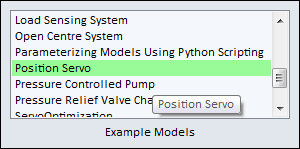
\includegraphics[width=0.5\textwidth]{gfx/optimization/openmodel.png}
%\end{figure}
%\FloatBarrier

%\icon{0}{gfx/Hopsan-Simulate.png}{Simulate current project (Ctrl-Shift-S)}

\end{enumerate}

\end{document}